\section{Multiplicative Updates for DL Training}

\begin{frame}{Thesis Contribution}
  Even though \textbf{multiplicative updates have several interesting properties}
  for neural networks and their hardware integration, \textbf{they are merely studied in
  the literature}.
  
  \begin{itemize}
    \item An \textbf{generic framework for alternative update rules}, allowing moderate
      the update rules for all well known optimization methods
    \item A \textbf{novel multiplicative update rule} that \textbf{accelerates} convergence and\textbf{ robustness} of training
    \item A \textbf{hybrid multiplicative-additive} update that \textbf{overcomes the limitations} of multiplicative updates
  \end{itemize}	
\end{frame}

\begin{frame}{Generic Optimization Framework for Alternative Updates}
\begin{algorithm}[H]
  \SetKwData{Left}{left}\SetKwData{This}{this}
  \SetKwData{Up}{up}\SetKwFunction{Union}{Union}
  \SetKwFunction{FindCompress}{FindCompress}
  \Begin{
      \While{\(t=1\) to \(T\) }{
        \(g_t = \nabla_{\theta}f_t(\theta_{t-1}) \) Gradients \\
        \(m_t = \phi_{t}(g_1,\ldots, g_t):\mathbb{R}^{t} \rightarrow \mathbb{R}
        \) Momentum \\
        \(l_t = \psi_{t}(g_1,\ldots, g_t): \mathbb{R}^{t} \rightarrow \mathbb{R}^{t}\) Adaptive Learning Rate \\
        \(\Delta\theta_t = \xi(\theta_{t-1}, m_t, l_t, \eta): \mathbb{R}^{t}
        \rightarrow \mathbb{R}\) Update Rule \\
      }
    }
    \caption{Generic Optimization Framework for Alternative Updates (GOFAU) \label{alg:optim}}    
\end{algorithm}
\end{frame}

\begin{frame}{Additive Optimization Methods}  
	\begin{table}
    \renewcommand{\arraystretch}{3.5}
    \begin{tabularx}{\linewidth}{l|c|c|c|c}
      & \textbf{SGD} & \textbf{Adagrad} & \textbf{Adam} & \textbf{RMSprop} \\
      \hline
      \(\phi_{t}(\cdot)\) & \(g_t\) & \(g_t\) &
                                                          \(\frac{(1-\beta_1)\sum_{i=1}^t\beta_1^{t-i}g_i}{1-\beta_1^t}\)
                             &  \(g_t\) \\
      \hline
      \(\psi_{t}(\cdot)\)    &  1  & \( \left( \sum_{i=1}^{t}g_i^2 \right)^{-1/2}\) &
                                                                 \(\sqrt{\frac{1-\beta_2^t}{(1-\beta_2)\sum_{i=1}^{t}\beta_2^{t-i}g_i^2}}\)
                                                          &
                                                            \(\sqrt{\frac{1-\beta_2^t}{(1-\beta_2)\sum_{i=1}^{t}\beta_2^{t-i}g_i^2}}\)\\
      \hline     
      \(\xi(\cdot)\) & \multicolumn{4}{c}{\cellcolor{blue!25}\(\eta m_t l_t\)}
    \end{tabularx}
  \end{table}
\end{frame}

\begin{frame}{Limitation of Additive Update}    
	
    \begin{equation*}
    \theta_t = \theta_{t-1} - \eta m_t l_t
  \end{equation*}
  
  \begin{itemize}
    \item \textbf{Depends on the gradient values} and the \textbf{learning rate}
    \item Extremely \textbf{sensitive to magnitude} of parameters
    \item Training difficulties when parameters are far from local or global
      minimum
    \item This exists profoundly when the \textbf{initialization is bad}
    \item Difficulties with default learning rate values
  \end{itemize}

\end{frame}

\begin{frame}{Proposed Multiplicative Update}
	\begin{table}
    \renewcommand{\arraystretch}{3.5}
    \begin{tabularx}{\linewidth}{l|c|c|c|c}
      & \textbf{SGD} & \textbf{Adagrad} & \textbf{Adam} & \textbf{RMSprop} \\
      \hline
      \(\phi_{t}(\cdot)\) & \(g_t\) & \(g_t\) &
                                                          \(\frac{(1-\beta_1)\sum_{i=1}^t\beta_1^{t-i}g_i}{1-\beta_1^t}\)
                                                          &  \(g_t\) \\ \hline
      \(\psi_{t}(\cdot)\)   & 1  & \( \left( \sum_{i=1}^{t}g_i^2 \right)^{-1/2}\) &
                                                                 \(\sqrt{\frac{1-\beta_2^t}{(1-\beta_2)\sum_{i=1}^{t}\beta_2^{t-i}g_i^2}}\)
                                                          &
                                                            \(\sqrt{\frac{1-\beta_2^t}{(1-\beta_2)\sum_{i=1}^{t}\beta_2^{t-i}g_i^2}}\)\\ \hline
      \(\xi(\cdot)\) & \multicolumn{4}{c}{\cellcolor{blue!25} \(|\theta_{t-1}|\tanh{\left(\eta_{in} m_t l_t \right)}\eta_{out}\)}

    \end{tabularx}
  \end{table}
\end{frame}

\begin{frame}{Benefits of Multiplicative Update Rule}
  \tikzstyle{na} = [baseline=-.5ex]
  
  \begin{itemize}[<+-| alert@+>]
  \item Normalize gradient 
    \tikz[na]\node [coordinate] (nCPP) {};
  \item Proportionally scales
    \tikz[na]\node [coordinate] (tps) {};
  \end{itemize}
  
	\begin{equation}
    \theta_{t} = \theta_{t-1} -
    \tikz[baseline]{\node[fill=blue!20,anchor=base] (mps) {$|\theta_{t-1}|$} ;}
    \tikz[baseline]{\node[fill=blue!20,anchor=base] (tL) {$\tanh$};}
    \tikz[baseline]{\node[fill=blue!20,anchor=base] (mml) {{$\left(\eta_{in} m_t l_t \right)$}};}
    \tikz[baseline]{\node[fill=blue!20,anchor=base] (mtu) {$\eta_{out}$};}
  \end{equation}

  \begin{tikzpicture}[overlay]
    \path[->]<1-> (nCPP) edge [bend left] (tL);
    \path[->]<2-> (tps) edge [bend left] (mps);
    \path[->]<3-> (bml) edge [bend right] (mml);
    \path[->]<4-> (btu) edge [bend right] (mtu);

        % \path[->]<2-> (nL) edge [bend left] (tL);
        % \path[->]<3-> (nPPP) edge [out=0, in=0] (tPPP);
        % \path[->]<4-> (nPP) edge [out=0, in=-90] (tPP);
  \end{tikzpicture}

  \begin{itemize}[<+-| alert@+>]
  \item Measures the scaling
    \tikz[na]\node [coordinate] (bml) {};
  \item Proportionally thresholds the update \tikz[na]\node [coordinate] (btu) {};
    \begin{itemize}
    \item \(\left[-\eta_{out}|\theta_{t-1}|, \eta_{out}|\theta_{t-1}|\right]\)
    \end{itemize}
  \item Preserves the sign of parameter
  \begin{itemize}
      \item \(\theta_{t}\theta_{t-1} \geq 0\)
    \end{itemize}
  \end{itemize}

\end{frame}

% \begin{frame}
% \tikzstyle{na} = [baseline=-.5ex]

% \begin{itemize}[<+-| alert@+>]
%     \item Class Prior Probability
%         \tikz[na]\node [coordinate] (nCPP) {};
%     \item Likelihood
%         \tikz[na]\node [coordinate] (nL) {};
% \end{itemize}

% \begin{equation*}
% \frac{
% \tikz[baseline]{\node[fill=blue!20,anchor=base] (tL) {$p(D|\theta)$};}
% \tikz[baseline]{\node[fill=red!20,anchor=base] (tCPP) {$p(\theta)$};}
% }
% {
% \tikz[baseline]{\node[fill=green!20,anchor=base] (tPPP) {$p(D)$};}
% }
% =
% \tikz[baseline]{\node[fill=yellow!20,anchor=base] (tPP) {$p(\theta | D)$};}
% \end{equation*}
% \begin{itemize}[<+-| alert@+>]
%     \item Predictor Prior Probability
%         \tikz[na]\node [coordinate] (nPPP) {};
%     \item Posterior probability
%         \tikz[na] \node[coordinate] (nPP) {};
% \end{itemize}

% \begin{tikzpicture}[overlay]
%         \path[->]<1-> (nCPP) edge [bend left] (tCPP);
%         \path[->]<2-> (nL) edge [bend left] (tL);
%         \path[->]<3-> (nPPP) edge [out=0, in=0] (tPPP);
%         \path[->]<4-> (nPP) edge [out=0, in=-90] (tPP);
% \end{tikzpicture}
% \end{frame}

\begin{frame}{Proposed Hybrid Update}
	\begin{table}
    \renewcommand{\arraystretch}{3.5}
    \begin{tabularx}{\linewidth}{l|c|c|c|c}
      & \textbf{SGD} & \textbf{Adagrad} & \textbf{Adam} & \textbf{RMSprop} \\
      \hline
      \(\phi_{t}(\cdot)\) & \(g_t\) & \(g_t\) &
                                                          \(\frac{(1-\beta_1)\sum_{i=1}^t\beta_1^{t-i}g_i}{1-\beta_1^t}\)
                                                          &  \(g_t\) \\ \hline
      \(\psi_{t}(\cdot)\)    & 1  & \( \left( \sum_{i=1}^{t}g_i^2 \right)^{-1/2}\) &
                                                                 \(\sqrt{\frac{1-\beta_2^t}{(1-\beta_2)\sum_{i=1}^{t}\bConvexeta_2^{t-i}g_i^2}}\)
                                                          &
                                                            \(\sqrt{\frac{1-\beta_2^t}{(1-\beta_2)\sum_{i=1}^{t}\beta_2^{t-i}g_i^2}}\)\\ \hline
      \(\xi(\cdot)\) & \multicolumn{4}{c}{\cellcolor{blue!25} \(\gamma\left(|\theta_{t-1}|\tanh{\left(\eta_{in} m_t l_t \right)}\eta_{out}\right) + (1-\gamma) \left(\eta m_t l_t\right)\)}
                                                                                                                                              
    \end{tabularx}
  \end{table}
\end{frame}

\begin{frame}{Proposed Hybrid Update}
  \begin{itemize}[<+-| alert@+>]
  \item Additive: Overcomes sign limitation \tikz[na]\node [coordinate] (tos) {};
  \item Acceleration and robustness  \tikz[na]\node [coordinate] (tar) {};
  \end{itemize}
  
	\begin{equation}
    \theta_{t} = \theta_{t-1} -
    \tikz[baseline]{\node[fill=blue!20,anchor=base] (mwra) { $\gamma$} ;}
    \tikz[baseline]{\node[fill=blue!20,anchor=base] (mar) { $\left(|\theta_{t-1}|\tanh{\left(\eta_{in} m_t l_t \right)}\eta_{out}\right) $} ;}
    +
    \tikz[baseline]{\node[fill=blue!20,anchor=base] (mwrb) { $(1-\gamma) $} ;}
    \tikz[baseline]{\node[fill=blue!20,anchor=base] (mos) { $ \left(\eta m_t l_t\right) $} ;}
  \end{equation}
  
  \begin{itemize}[<+-| alert@+>]
    \item Weights relative \tikz[na]\node [coordinate] (bwra) {}; contribution \tikz[na]\node [coordinate] (bwrb) {};
    \end{itemize}

    \begin{tikzpicture}[overlay]
      \path[->]<1-> (tos) edge [bend left] (mos);
      \path[->]<2-> (tar) edge [bend left] (mar);
      \path[->]<3-> (bwra) edge [bend] (mwra);
      \path[->]<3-> (bwrb) edge [bend right] (mwrb);
    \end{tikzpicture}
\end{frame}

\begin{frame}{Experimental Evaluation: An Example}
	\begin{figure}
    \centering
    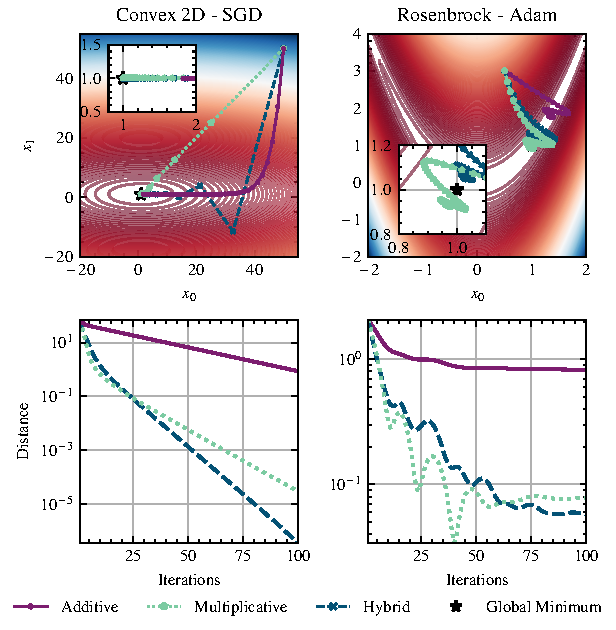
\includegraphics[width=0.75\linewidth]{./sections/5_mult/imgs/selection_convex.pdf}
    % \caption{The top Figures demonstrate the optimization process for Convex 2D
    %   and Rosenbrock tasks alternative updates for SGD and Adam optimizers,
    %   respectively. The bottom Figures report the Euclidean distance between the
    %   parameters and the actual global minimum. }
    \label{fig:convex_opt}
\end{figure}
\end{frame}


% \begin{frame}{Experimental Results}
% 	\begin{table}[]
%     \centering
%      \caption{Distance from global minimum after 100 iterations using the best training configuration}
%     \label{tab:tune_convex}
%     \resizebox{0.8\linewidth}{!}{\begin{tabular}{l|c|c|c}
%          \toprule
%          Optimizer & \mythead{\normalfont Baseline\\\normalfont(Additive)} & \mythead{\textbf{GOFAU}\\\textbf{(Multiplicative)}} & \mythead{\textbf{GOFAU}\\\textbf{(Hybrid)}} \\
%          \midrule
%          \multicolumn{4}{c}{\textbf{Convex 2D} \textit{(69.26)}}\\ \midrule
%          SGD & \(8.61\times10^{-1}\) & \(2.92\times10^{-5}\) & \(\bm{3.57\times10^{-7}}\)  \\
%          Adagrad & \(5.80\times10^{-4}\) & \(1.35\times10^{-4}\) & \(\underline{\bm{1.68\times10^{-7}}}\) \\
%          Adam & \(3.75\times10^{-2}\) & \(7.44\times10^{-3}\) & \(\bm{4.47\times10^{-3}}\)  \\
%          RMSProp & \(1.82\times10^{-5}\) & \(7.58\times10^{-6}\) & \(\underline{\bm{1.68\times10^{-7}}}\)  \\ \midrule
%          \multicolumn{4}{c}{\textbf{Rosenbrock} \textit{(2.06)}}\\ \midrule
%          SGD & \(1.38 \times 10^{0}\) & \(7.70\times10^{-2}\) & \(\bm{2.04\times10^{-2}}\) \\
%          Adagrad & \(4.60 \times 10^{-1}\) & \(1.88\times10^{-1}\) &  \(\underline{\bm{1.26\times10^{-2}}}\) \\
%          Adam & \(8.24\times 10^{-1}\) & \(7.84\times10^{-2}\) & \(\bm{5.73\times10^{-2}}\) \\
%          RMSProp & \(4.58\times10^{-1}\) & \(1.85\times10^{-1}\)  & \(\bm{5.06\times10^{-2}}\)  \\
%         \bottomrule
%     \end{tabular}}
% \end{table}
% \end{frame}



% \begin{frame}{Experimental Evaluation: Robustness}
% 	\begin{table*}
%     \centering
%     \caption{Evaluation of optimizers on 100 randomly drawn configurations. The relative Euclidean distance the parameters and the actual global minimum is reported }
%     \label{tab:convex_res}
%     \resizebox{\linewidth}{!}{\begin{tabular}{l|l|l|l}
%          \toprule
%          Optimizer & \mythead{\normalfont Baseline\\\normalfont(Additive)} & \mythead{\textbf{GOFAU}\\\textbf{(Multiplicative)}} & \mythead{\textbf{GOFAU}\\\textbf{(Hybrid)}} \\
%          \midrule
%          \multicolumn{4}{c}{\textbf{Convex 2D}}\\ \midrule
%          SGD & \(1.48\times10^{-2}\pm{8.06\times10^{-3}}\) & \(1.82\times10^{-3}\pm{5.17\times10^{-3}}\) & \(\bm{8.37\times10^{-4} \pm{2.35\times10^{-3}}}\)  \\
%          Adagrad & \(7.61\times10^{-5}\pm{1.67\times10^{-4}}\) & \(2.30\times10^{-3}\pm{7.17\times10^{-3}}\) & \(\underline{\bm{1.79\times10^{-9} \pm{1.34\times10^{-9}}}}\) \\
%          Adam & \(4.28\times10^{-3}\pm{4.28\times10^{-3}}\) & \(3.95\times10^{-3}\pm{4.88\times10^{-3}}\) & \(\bm{1.26\times10^{-3}\pm{1.45\times10^{-3}}}\)  \\
%          RMSProp & \(8.26\times10^{-6}\pm{2.33\times10^{-5}}\) & \(2.24\times10^{-3}\pm{2.24\times10^{-3}}\) & \(\bm{2.01\times10^{-8}\pm{9.58\times10^{-8}}}\)  \\ \midrule
%          \multicolumn{4}{c}{\textbf{Rosenbrock}}\\ \midrule
%          SGD & \(5.88\times10^{-1}\pm{2.19\times10^{-1}}\) & \(1.75\times10^{-1}\pm{2.36\times10^{-1}}\) & \(\underline{\bm{7.42\times10^{-2}\pm{1.53\times10^{-1}}}}\) \\
%          Adagrad & \(3.53\times10^{-1}\pm{3.59\times10^{-1}}\) & \(2.03\times10^{-1}\pm{2.13\times10^{-1}}\) &  \(\bm{1.98\times10^{-1}\pm{2.68\times10^{-1}}}\) \\
%          Adam & \(4.12\times10^{-1}\pm{1.69\times10^{-1}}\) & \(1.68\times10^{-1}\pm{2.55\times10^{-1}}\) & \(\bm{1.48\times10^{-1}\pm{1.58\times10^{-1}}}\) \\
%          RMSProp & \(3.16\times10^{-1}\pm{3.08\times10^{-1}}\) & \(1.43\times10^{-1}\pm{1.67\times10^{-1}}\)  & \(\bm{2.01\times10^{-1}\pm{2.51\times10^{-1}}}\)  \\
%         \bottomrule
%     \end{tabular}}
% \end{table*}
% \end{frame}

\begin{frame}{Experimental Evaluation: Robustness}
	\begin{figure}
    \centering
    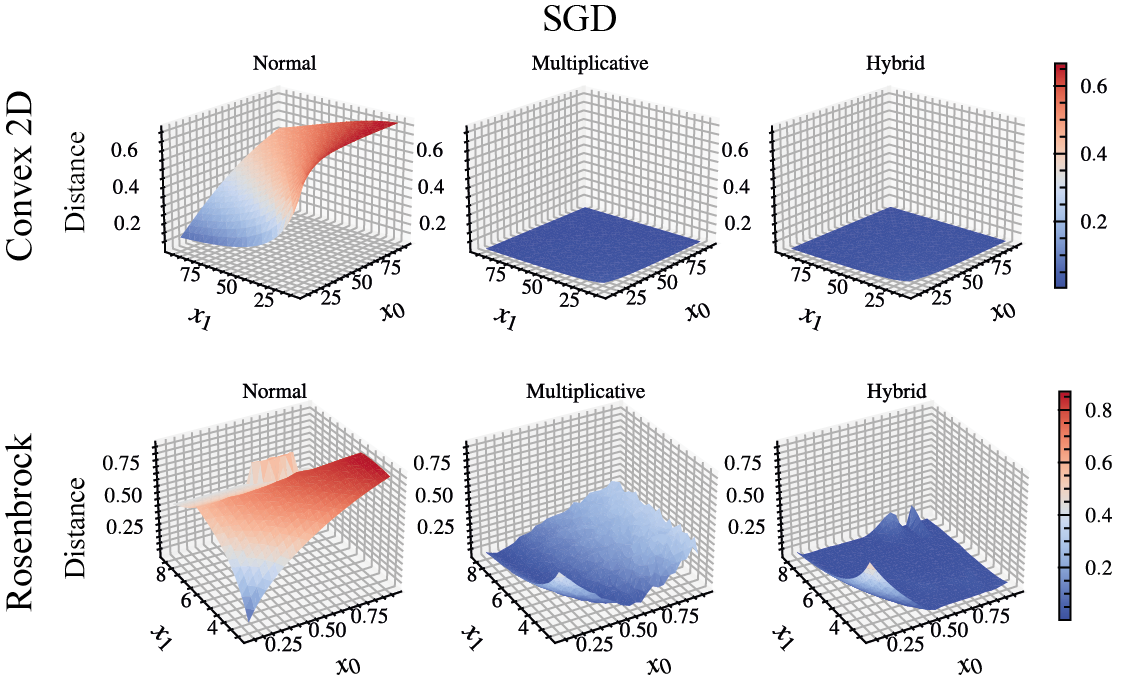
\includegraphics[width=\textwidth]{./sections/5_mult/imgs/surface_plot_v2.png}
    \caption{Distance from global minimum of the evaluated update rules applying
      SGD optimization methods in two optimization tasks. }
    \label{fig:surface_plot}
\end{figure}
\end{frame}


% \begin{frame}{CIFAR100 - ResNet18}
% 	\begin{figure}
%     \centering
%     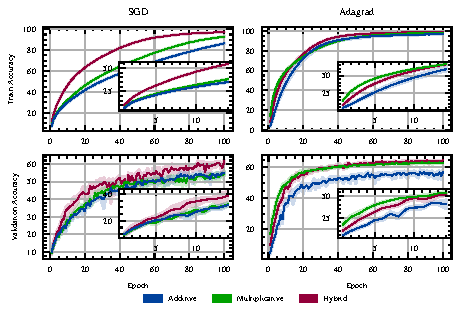
\includegraphics[width=\linewidth]{./sections/5_mult/imgs/230309_cifar100_resnet18.pdf} 
%     % \caption{Training and validation accuracy during training applying ResNet18
%     %   architecture on CIFAR100 dataset using default configurations for both
%     %   task and optimizers }
%     \label{fig:cifar100}
%   \end{figure}
% \end{frame}

% \begin{frame}{Tiny ImageNet - ResNet18}
%   \begin{figure}[t]{\linewidth}
%         \centering
%         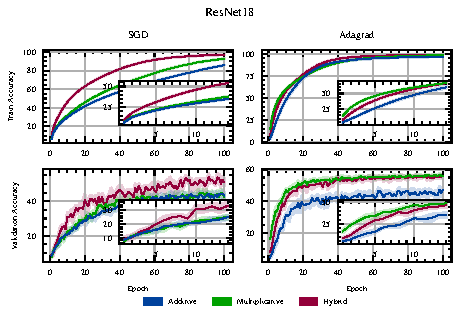
\includegraphics[width=\linewidth]{./sections/5_mult/imgs/230313_tiny_imagenet_resnet18.pdf}
%       %   \caption{Training and validation accuracy during training on Tiny ImageNet
%       % dataset using default configurations for both task and optimizers}
%     \end{figure}
% \end{frame}

\begin{frame}{Experimental Evaluation: Tiny ImageNet - ResNet18}
      \begin{figure}[t]{\linewidth}
        \centering
        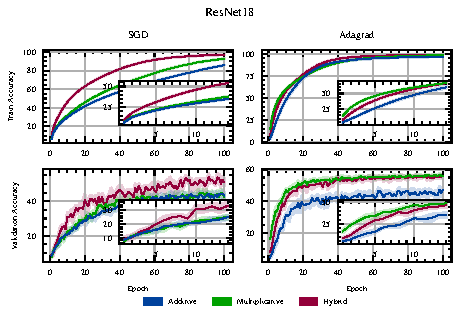
\includegraphics[width=\linewidth]{./sections/5_mult/imgs/230313_tiny_imagenet_resnet18.pdf}
      %   \caption{Training and validation accuracy during training on Tiny ImageNet
      % dataset using default configurations for both task and optimizers}
    \end{figure}
\end{frame}

\begin{frame}{Experimental Evaluation: CIFAR100 - ResNet18}
    \begin{table}
  \centering
    \begin{tabular}{l|ccc}
      \toprule
      Optimizer & Final. Acc. $\uparrow$ \\
      \midrule
      \textbf{Hybrid Adam} & $67.10\pm{0.35}$\\
      \textbf{Hybrid RMSprop} & $65.15\pm{0.90}$\\
      \textbf{Hybrid Adagrad} & $64.54\pm{0.74}$ \\
      Nero & $64.23\pm{0.81}$ \\
      Fromage & $63.42\pm{0.82}$ \\
      \textbf{Mult. Adagrad} & $62.98\pm{0.45}$ \\
      \textbf{Hybrid SGD} & $61.58\pm{1.11}$ \\
      LAMB & $61.50\pm{0.64}$  \\
      \textbf{Mult. Adam} & $61.44\pm{0.50}$ \\
      \textbf{Mult. RMSprop} & $61.12\pm{1.27}$ \\
      SignSGD & $56.26\pm{1.48}$ \\
      \textbf{Mult. SGD} & $54.52\pm{1.59}$ \\
      MAdam & $52.53\pm{5.67}$  \\

      \bottomrule
    \end{tabular}
  \end{table}
\end{frame}

\begin{frame}{Publication}
\begin{itemize}
    \item Main Journal Publications
     \begin{itemize}
        \item {\scriptsize \textbf{Kirtas, M.}, Passalis, N. and Tefas, A., 2024. \href{https://www.sciencedirect.com/science/article/abs/pii/S0925231224001231}{Multiplicative update rules for accelerating deep learning training and increasing     robustness.} Neurocomputing, Elsevier}
    \end{itemize}
    \item Main Conferences Publications 
    \begin{itemize} 
        \item {\scriptsize \textbf{Kirtas, M.}, Passalis, N., Tefas, A., 2025, Multiplicative Stochastic Gradient Descent for fast and robust deep learning training, \textit{Accepted at International Joint Conference on Neural Networks (IJCNN) 2025 }}
          \item {\scriptsize \textbf{Kirtas, M.}, Passalis, N. and Tefas, A., 2024, December. \href{https://link.springer.com/chapter/10.1007/978-3-031-78110-0_21}{Multiplicative RMSprop Using Gradient Normalization for Learning Acceleration.}In International Conference on Pattern Recognition}
          \item {\scriptsize \textbf{Kirtas, M.}, Passalis, N., Tefas, A., 2025, Fast and robust training of deep learning models with multiplicative Adagrad, IEEE International Workshop on Machine Learning for Signal Processing (MLSP), \textit{Accepted}}
    \end{itemize}
\end{itemize}
\end{frame}
